\chapter{Hojas de universo, rotación de Wick y dualidad entre canales}

\lectureoverview{Una partícula recorre una línea de universo; una cuerda barre una hoja de universo. Cuantizar cualquiera de estos objetos requiere sumar sobre las historias posibles, pero la suma lorentziana es oscilatoria y difícil de definir. Al convertir el tiempo de la hoja de universo en una coordenada imaginaria, se obtiene una teoría euclídea regida por la ecuación de Laplace. Su simetría conforme permite entonces transformar la superficie con cortes de una interacción entre cuatro cuerdas en un disco con cuatro inserciones en el borde, donde se hace visible la simetría entre los canales directo y cruzado.}

\section{De la línea de universo a la suma sobre historias}

Empecemos con una partícula libre. En mecánica no relativista, su posición es una función \(\mathbf x(t)\) y, tomando la masa igual a uno, su acción es \begin{equation}
  S_{\mathrm{NR}}[\mathbf x]
  =\frac12\int_{t_1}^{t_2}\dot{\mathbf x}^{\,2}\,dt.
  \label{eq:l07-nr-action}
\end{equation} Para una descripción relativista, resulta más natural reunir el tiempo y el espacio en un vector, \(X^\mu(\tau)\), parametrizado a lo largo de la trayectoria mediante \(\tau\). La expresión cuadrática correspondiente es \begin{equation}
  S_{\mathrm{rel}}[X]
  =\frac12\int_{\tau_1}^{\tau_2}
  \frac{dX^\mu}{d\tau}\frac{dX_\mu}{d\tau}\,d\tau.
  \label{eq:l07-rel-action}
\end{equation} Los índices superiores e inferiores codifican la diferencia de signo lorentziana entre el tiempo y el espacio. \editorialnote{La acción relativista cuadrática se utiliza con una parametrización fija de la línea de universo. La alternativa manifiestamente invariante bajo reparametrizaciones es proporcional a la longitud propia, que se menciona más adelante en la conferencia.}

\begin{figure}[H]\centering
  \includegraphics[width=0.72\textwidth]{lecture_07_figure_01.png}\caption{Las acciones no relativista y relativista cuadrática, escritas juntas en la pizarra.}\lectureframe{00:03:35}\label{fig:l07-particle-actions}\end{figure}

Clásicamente, se fijan los extremos y se varía la trayectoria. La partícula libre sigue entonces una línea de universo recta con velocidad constante. La mecánica cuántica plantea otra pregunta. No selecciona una única trayectoria entre los extremos; pregunta cuál es la amplitud de que la partícula comience en un punto y se detecte en el otro. Cada trayectoria intermedia contribuye con una fase, \begin{equation}
  K(2,1)=\int_{X(1)}^{X(2)}\!\mathcal D X\,
  e^{iS[X]}.
  \label{eq:l07-feynman-integral}
\end{equation} La integral funcional es una integral sobre un espacio infinito-dimensional de trayectorias, no la integral ordinaria que ya aparece dentro de la acción.

\begin{figure}[H]\centering
  \includegraphics[width=0.72\textwidth]{lecture_07_figure_02.png}\caption{Una trayectoria representativa y la fase que se le asigna antes de efectuar la suma sobre todas las trayectorias.}\lectureframe{00:06:21}\label{fig:l07-path-integral-board}\end{figure}

En lenguaje relativista, esta amplitud entre dos puntos es un propagador. En una interacción, se unen varios segmentos de líneas de universo. Se suman sus acciones, se integra sobre los puntos de unión y se suman los diagramas con las partículas externas requeridas. Así pues, la conocida expansión en diagramas de Feynman ya está implícita en la instrucción de sumar sobre las historias.

Aquí, el símbolo \(S\) denotará una acción. No guarda relación ni con la entropía ni con la variable de Mandelstam \(s\) que se usa cerca del final de la conferencia. La notación compartida es tradicional, pero poco esclarecedora.

\section{Girar el tiempo hacia una dirección imaginaria}

Hay un problema inmediato con \eqref{eq:l07-feynman-integral}. Cada factor \(e^{iS}\) tiene módulo uno. Por tanto, una trayectoria que se aleja mucho y oscila intensamente y la línea recta clásica entran con el mismo peso absoluto; solo difieren sus fases. La interferencia destructiva recupera el comportamiento clásico, pero no convierte la integral formal en un objeto ordinario convergente.

Introduzcamos un nuevo parámetro \(s\) mediante \begin{equation}
  \tau=\alpha s,
  \qquad
  d\tau=\alpha\,ds,
  \qquad
  \frac{dX}{d\tau}=\frac{1}{\alpha}\frac{dX}{ds}.
\end{equation} Entonces, la acción cuadrática se reescala así: \begin{equation}
  \frac12\int d\tau
  \left(\frac{dX}{d\tau}\right)^2
  =
  \frac{1}{2\alpha}\int ds
  \left(\frac{dX}{ds}\right)^2.
  \label{eq:l07-rescaled-action}
\end{equation} Elegir el contorno correspondiente a \(\alpha=-i\) transforma el peso oscilatorio en \begin{equation}
  e^{iS}
  \longrightarrow
  \exp\!\left[-\frac12\int ds
  \left(\frac{dX}{ds}\right)^2\right]
  =e^{-S_E}.
  \label{eq:l07-euclidean-particle}
\end{equation}

\begin{figure}[H]\centering
  \includegraphics[width=0.66\textwidth]{lecture_07_figure_03.png}\caption{El peso euclídeo de la partícula tras la sustitución de tiempo imaginario; el exponente es real y no positivo.}\lectureframe{00:16:20}\label{fig:l07-particle-wick}\end{figure}

Una trayectoria que se aleja mucho y regresa, o que oscila rápidamente sin recorrer una gran distancia, tiene un valor grande y positivo de \(S_E\) y queda suprimida exponencialmente. El resultado es una integral de tipo Wiener, para la cual existe una teoría de la convergencia rigurosa. Los extremos heredados de valores reales de \(\tau\) se encuentran sobre un contorno imaginario de \(s\). En la práctica, se evalúa el objeto euclídeo en su dominio de convergencia y después se continúa analíticamente la respuesta hasta recuperar las variables lorentzianas físicas. Esta operación es la rotación de Wick: para el cálculo se ha girado el tiempo hacia una dirección imaginaria, no se lo ha descartado.

\section{De las líneas de universo a las hojas de universo}

Una partícula puntual tiene una línea de universo. Una cuerda abierta barre una cinta, y una cuerda cerrada barre un tubo. Las coordenadas \((\sigma,\tau)\) señalan puntos de esta hoja de universo bidimensional, mientras que \begin{equation}
  X^\mu=X^\mu(\sigma,\tau)
  \label{eq:l07-embedding}
\end{equation} da la posición en el espacio-tiempo del punto señalado. Conocer todas las funciones \(X^\mu\) especifica la historia completa de la cuerda.

La acción cuadrática lorentziana de la hoja de universo tiene la misma estructura de energía cinética menos energía potencial que la de una cuerda vibrante ordinaria: \begin{equation}
  S_{\mathrm{ws}}[X]
  =\frac{T_s}{2}\int d\tau\,d\sigma\,
  \left[
    \partial_\tau X^\mu\partial_\tau X_\mu
    -
    \partial_\sigma X^\mu\partial_\sigma X_\mu
  \right].
  \label{eq:l07-lorentzian-worldsheet}
\end{equation} La tensión total \(T_s\) fija la escala; en esta conferencia se omite mientras se presta atención a la estructura de las derivadas.

\begin{figure}[H]\centering
  \includegraphics[width=0.72\textwidth]{lecture_07_figure_04.png}\caption{La acción lorentziana de la hoja de universo para \(X^\mu(\sigma,\tau)\), con el signo de energía cinética menos energía potencial.}\lectureframe{00:24:26}\label{fig:l07-worldsheet-action}\end{figure}

La amplitud de la cuerda se obtiene exponenciando esta acción y sumando sobre todas las superficies que conectan las configuraciones iniciales y finales prescritas de la cuerda: \begin{equation}
  \mathcal A=\int\mathcal D X\,e^{iS_{\mathrm{ws}}[X]}.
  \label{eq:l07-surface-integral}
\end{equation} La misma regla describe dos cuerdas que se convierten en dos, en tres o en cualquier otra configuración externa permitida. La suma incluye también distintas topologías de la hoja de universo. Añadir agujeros es el equivalente, en teoría de cuerdas, a añadir órdenes de bucle en una expansión de diagramas de partículas puntuales.

\begin{figure}[H]\centering
  \includegraphics[width=0.66\textwidth]{lecture_07_figure_05.png}\caption{Una superficie que conecta varias cuerdas externas, con un agujero que representa otra topología de la hoja de universo.}\lectureframe{00:27:14}\label{fig:l07-surface-topology}\end{figure}

\begin{classroomqa}\audiencequestion{Para un electrón puntual, ¿se anula simplemente la derivada respecto de \(\sigma\)? \lecturetimestamp{00:27:56}}\lecturerresponse{Una partícula puntual ni siquiera tiene coordenada \(\sigma\). Aun así, los dibujos están relacionados: cuando los estados externos son ligeros en comparación con la escala de cuerdas y las energías del proceso son bajas, las amplitudes de cuerdas reproducen los diagramas de Feynman ordinarios de partículas puntuales. Ese límite va mucho más allá de hacer que una derivada se anule.}\end{classroomqa}

La integral sobre superficies tiene el mismo problema de convergencia que la integral sobre trayectorias. Tras aplicar la rotación de Wick al tiempo de la hoja de universo, su forma euclídea estable es \begin{equation}
  \begin{aligned}
    S_{E,\mathrm{ws}}[X]
    &=\frac{T_s}{2}\int d\tau\,d\sigma\,
      \left[
        \partial_\tau X^\mu\partial_\tau X_\mu
        +\partial_\sigma X^\mu\partial_\sigma X_\mu
      \right],\\
    \mathcal A_E&=\int\mathcal D X\,e^{-S_{E,\mathrm{ws}}}.
  \end{aligned}
  \label{eq:l07-euclidean-worldsheet}
\end{equation} Ahora ambas derivadas aparecen con el mismo signo positivo. Una superficie que vibra violentamente o está muy estirada tiene una acción euclídea grande y queda suprimida.

\begin{figure}[H]\centering
  \includegraphics[width=0.72\textwidth]{lecture_07_figure_06.png}\caption{La densidad euclídea positiva de la hoja de universo después de rotar \(\tau\) a tiempo imaginario.}\lectureframe{00:34:29}\label{fig:l07-worldsheet-wick}\end{figure}

También existe una formulación geométricamente directa. A una partícula relativista se le puede asignar una acción proporcional a la longitud propia de su trayectoria; a una cuerda, una acción proporcional al área de su hoja de universo en el espacio-tiempo. Esta última es la acción de Nambu--Goto. La forma cuadrática de la hoja de universo que se usa aquí se denomina convencionalmente forma de Polyakov y resulta mucho más sencilla para el cálculo presente. \editorialnote{La conferencia incluye una discusión humorística sobre la atribución histórica de los nombres y menciona también la acción de Liouville, relacionada con ella, y las condiciones de contorno de Dirichlet. Para la derivación no hace falta reivindicar ninguna prioridad: solo se usa la equivalencia entre las formulaciones mediante el área y la métrica auxiliar.}

\section{La ecuación euclídea del movimiento}

Las coordenadas \(\sigma\) y \(\tau\) son solo etiquetas sobre la hoja. Así que la siguiente pregunta es inevitable: ¿qué cambios de etiquetas dejan invariante la teoría? La respuesta se ve más fácilmente a partir de la ecuación del movimiento. Al variar \eqref{eq:l07-euclidean-worldsheet} se obtiene, componente a componente, \begin{equation}
  \partial_\tau^2X^\mu+\partial_\sigma^2X^\mu=0.
  \label{eq:l07-laplace}
\end{equation} Antes de la rotación de Wick, el signo relativo es negativo y se trata de una ecuación de ondas. En signatura euclídea, ambos signos son positivos, por lo que se trata de la ecuación de Laplace bidimensional.

\begin{classroomqa}\audiencequestion{¿Es esta la ecuación de un tambor vibrante?\lecturetimestamp{00:41:50}}\lecturerresponse{Está estrechamente relacionada, pero un tambor vibrante también tiene una coordenada de tiempo real y, por tanto, obedece una ecuación de ondas. La ecuación de aquí es la ecuación de Laplace euclídea. El potencial electrostático en una región sin cargas es un ejemplo familiar más directo.}\end{classroomqa}

\begin{classroomqa}\audiencequestion{La acción contiene primeras derivadas. ¿Por qué su ecuación contiene segundas derivadas? \lecturetimestamp{00:42:44}}\lecturerresponse{Al variar un término cuadrático en una primera derivada e integrar por partes, una derivada pasa a actuar sobre esa primera derivada. Es la versión para campos de que \(\dot x^{\,2}\) en una acción produce \(\ddot x\) en la ecuación del movimiento.}\end{classroomqa}

\begin{figure}[H]\centering
  \includegraphics[width=0.68\textwidth]{lecture_07_figure_07.png}\caption{La ecuación de Laplace con signos positivos y la primera línea discreta que se usa para interpretar sus segundas derivadas.}\lectureframe{00:43:30}\label{fig:l07-laplace-board}\end{figure}

Para visualizar la geometría, discreticemos primero una coordenada con separación \(\epsilon\). Una primera derivada es una diferencia entre puntos vecinos, mientras que una segunda derivada es una diferencia entre diferencias de puntos vecinos: \begin{equation}
  \frac{d^2X}{ds^2}\bigg|_{2}
  \longrightarrow
  \frac{X(3)-2X(2)+X(1)}{\epsilon^2}.
  \label{eq:l07-second-difference}
\end{equation}

\begin{figure}[H]\centering
  \includegraphics[width=0.72\textwidth]{lecture_07_figure_08.png}\caption{La línea numerada, un pequeño fragmento de retícula y el desarrollo en diferencias finitas de una segunda derivada.}\lectureframe{00:45:51}\label{fig:l07-finite-difference-board}\end{figure}

Ahora discreticemos el plano \((\sigma,\tau)\). Denotemos por \(1,2,3,4\) los cuatro vecinos más próximos de un punto central \(5\). La ecuación \eqref{eq:l07-laplace} se convierte en \begin{equation}
  X(1)+X(2)+X(3)+X(4)-4X(5)=0,
\end{equation} o bien \begin{equation}
  X(5)=\frac14\bigl[X(1)+X(2)+X(3)+X(4)\bigr].
  \label{eq:l07-mean-value}
\end{equation}

\begin{figure}[H]\centering
  \includegraphics[width=0.72\textwidth]{lecture_07_figure_09.png}\caption{La ecuación bidimensional completa en diferencias finitas: el valor central es igual al promedio de sus cuatro vecinos.}\lectureframe{00:48:26}\label{fig:l07-mean-value-board}\end{figure}

Esta propiedad del valor medio se cumple para un cuadrado infinitesimal con cualquier orientación. Es el contenido geométrico local de la ecuación de Laplace y el vínculo con la simetría conforme.

\section{Coordenadas conformes}

Consideremos un cambio de \((\sigma,\tau)\) a \((\sigma',\tau')\). Una deformación general transforma un cuadrado pequeño en un cuadrilátero cualquiera. Las transformaciones especiales que nos interesan aquí llevan cada cuadrado infinitesimal a otro cuadrado infinitesimal, quizá rotado y reescalado. De manera equivalente, conservan los ángulos con que se cortan las curvas. Son las transformaciones conformes.

\begin{figure}[H]\centering
  \includegraphics[width=0.68\textwidth]{lecture_07_figure_10.png}\caption{Un cuadrado local se transforma en otra figura pequeña; se comprueba si se conservan sus ángulos.}\lectureframe{00:53:25}\label{fig:l07-conformal-board}\end{figure}

\begin{classroomqa}\audiencequestion{Si se conservan los ángulos, ¿la transformación consiste básicamente solo en una rotación? \lecturetimestamp{00:53:31}}\lecturerresponse{Solo localmente, e incluso en ese caso se permite también un cambio común de escala. La rotación local y el factor de escala pueden variar de un punto a otro, de modo que la cuadrícula de coordenadas puede curvarse, expandirse en una región y contraerse en otra, conservando las formas infinitesimales.}\end{classroomqa}

Una aplicación que conserva los ángulos no tiene por qué conservar el tamaño. Si también se conservara el tamaño en todas partes, las posibilidades se reducirían a la clase mucho más restringida de movimientos rígidos: traslaciones y rotaciones. En cambio, las aplicaciones conformes conservan la forma local. Por eso una proyección cartográfica puede preservar la forma de una isla pequeña y, aun así, distorsionar mucho su área.

\begin{classroomqa}\audiencequestion{¿Decir que una aplicación es conforme equivale a decir que el sistema de coordenadas es plano? \lecturetimestamp{00:55:35}}\lecturerresponse{No. La planitud y la conformidad son propiedades distintas. Una aplicación conforme puede utilizar líneas de coordenadas curvas; lo que conserva es el ángulo entre curvas que se cortan. Una proyección cartográfica de tipo Mercator es un ejemplo conocido que preserva la forma local con una distorsión considerable de la escala.}\end{classroomqa}

En dos dimensiones, las transformaciones requeridas se generan localmente mediante funciones analíticas de una coordenada compleja \begin{equation}
  z=\sigma+i\tau.
\end{equation} Los bordes finitos pueden cambiar de aspecto de manera drástica. Una región cuadrada puede transformarse en una región lisa, de modo que las esquinas originales se envíen a puntos ordinarios del nuevo borde y no a sus puntos más destacados visualmente. No hay contradicción: la conformidad es una condición local en el interior, y la aplicación conserva los ángulos infinitesimales allí donde es regular.

\begin{classroomqa}\audiencequestion{¿Es esta libertad de coordenadas la razón por la que se podía elegir de forma simétrica el diagrama anterior de unión--separación?\lecturetimestamp{00:56:32}}\lecturerresponse{Sí. La misma libertad conforme que conserva las ecuaciones de la hoja de universo nos permite reemplazar la incómoda franja de interacción por un dominio más simétrico. La libertad restante no elimina el parámetro físico de unión--separación; lo representa de nuevo como la posición relativa de las inserciones en el borde.}\end{classroomqa}

\section{La hoja con cortes y el disco}

Volvamos a la dispersión de cuatro cuerdas. Entran dos cuerdas abiertas, se unen sus extremos, la cuerda resultante se propaga y, más tarde, se divide. Dibujado como una hoja de universo plana, el proceso es una franja infinita con un corte en cada extremo. La separación \(\tau_0\) entre las puntas de los cortes es el tiempo de vida de la cuerda intermedia, y la amplitud se integra sobre ese parámetro.

\begin{figure}[H]\centering
  \includegraphics[width=0.72\textwidth]{lecture_07_figure_11.png}\caption{La franja con dos cortes representa dos cuerdas abiertas que se unen, se propagan juntas y vuelven a separarse.}\lectureframe{01:00:20}\label{fig:l07-slit-strip}\end{figure}

Tras la euclidianización, los campos de inmersión en esta región satisfacen la ecuación de Laplace. Por tanto, la invariancia conforme permite transformar la franja con cortes en un disco. Para visualizar la topología, se puede foliar el disco con círculos concéntricos y deformar continuamente esas curvas cerradas hasta que recubran la región con cortes. Bajo esta aplicación, los extremos en el infinito se convierten en puntos excepcionales del borde.

\begin{figure}[H]
  \centering
  \includegraphics[width=0.72\textwidth]{lecture_07_figure_12.png}
  \medskip

\begin{adjustbox}{max width=\linewidth}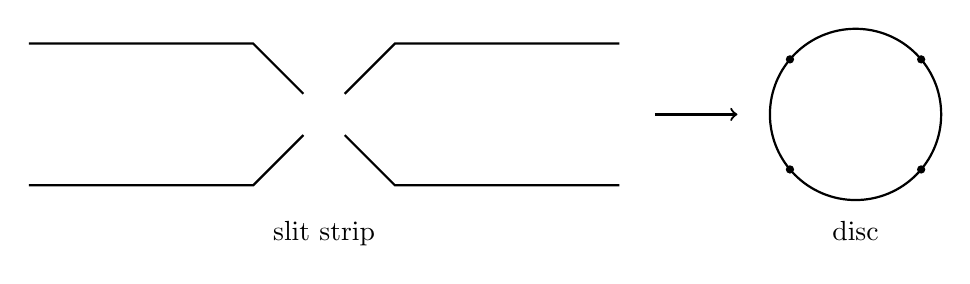
\begin{tikzpicture}[x=0.75cm,y=0.75cm]
    \draw[thick] (-5,1.2) -- (-1.2,1.2) -- (-0.35,0.35);
    \draw[thick] (-5,-1.2) -- (-1.2,-1.2) -- (-0.35,-0.35);
    \draw[thick] (0.35,0.35) -- (1.2,1.2) -- (5,1.2);
    \draw[thick] (0.35,-0.35) -- (1.2,-1.2) -- (5,-1.2);
    \draw[->,thick] (5.6,0) -- (7.0,0);
    \draw[thick] (9.0,0) circle (1.45);
    \foreach \a in {40,140,220,320} \fill (9.0,0) ++(\a:1.45) circle (1.5pt);
    \node[below] at (0,-1.65) {slit strip};
    \node[below] at (9.0,-1.65) {disc};
  \end{tikzpicture}\end{adjustbox}\caption{Comparación de las curvas de nivel de la pizarra y esquema limpio de la aplicación conforme de la franja con cortes a un disco. Los cuatro extremos externos se convierten en cuatro puntos especiales del borde.}\lectureframe{01:04:46}\label{fig:l07-strip-to-disc}\end{figure}

Los estados externos no se pierden en este cambio de coordenadas. En los cuatro puntos excepcionales hay que insertar el momento, el tipo de partícula y el nivel de oscilador. Los objetos formales que transportan esa información son los operadores vértice. Su construcción detallada se deja para más adelante, pero su función ya está clara: convierten una integral de caminos sobre la hoja de universo, por lo demás homogénea, en un experimento de dispersión especificado.

Tras usar transformaciones conformes del disco para llevar tres puntos del borde a posiciones de referencia convenientes, queda una posición relativa real. Se puede representar mediante la razón doble de los cuatro puntos ordenados del borde. Esta es la versión en el disco del antiguo tiempo de vida \(\tau_0\).

\begin{figure}[H]\centering
  \includegraphics[width=0.62\textwidth]{lecture_07_figure_13.png}\caption{Cuatro puntos de inserción en el borde del disco. La libertad conforme elimina todos los grados de libertad salvo un módulo real de su configuración ordenada.}\lectureframe{01:10:55}\label{fig:l07-four-points}\end{figure}

Por tanto, la integral sobre el tiempo de vida no ha desaparecido. Se ha convertido en una integral sobre el módulo restante. Con la coordenada convencional \(0<z<1\), la integral de cuatro puntos de cuerda abierta adopta la misma forma que en la conferencia anterior: \begin{equation}
  \mathcal A(s,t)\propto
  \int_0^1 z^{-s-1}(1-z)^{-t-1}\,dz.
  \label{eq:l07-modulus-integral}
\end{equation}

\section{Dos límites de una misma superficie}

En un extremo del espacio de módulos, los dos puntos de inserción asociados al par entrante se acercan entre sí. En las coordenadas de la franja con cortes, esto corresponde a un intervalo largo entre la unión y la separación: una cuerda intermedia del canal directo se propaga durante mucho tiempo. En el otro extremo, se acerca otro par de puntos vecinos. Entonces, la misma superficie se interpreta de manera natural como un intercambio en el canal cruzado. En la franja, estas descripciones parecen no tener relación, pero son límites vecinos de borde de una misma integral sobre el disco.

Volviendo a la convención de signatura mayoritariamente positiva de la conferencia anterior, \begin{equation}
  -s=(k_1+k_2)^2,
  \qquad
  -t=(k_1+k_3)^2.
  \label{eq:l07-mandelstam}
\end{equation} El límite directo organiza los polos en \(s\); el límite cruzado organiza los polos en \(t\). \editorialnote{Cerca del final de la conferencia, la pizarra usa un signo abreviado para los invariantes de Mandelstam y, al mismo tiempo, identifica \(s\) con la energía positiva del centro de masas al cuadrado. La ecuación \eqref{eq:l07-mandelstam} mantiene la convención de signatura mayoritariamente positiva establecida en la conferencia 6.}

\begin{figure}[H]\centering
  \includegraphics[width=0.62\textwidth]{lecture_07_figure_14.png}\caption{Los diagramas de los dos canales: propagación prolongada en una orientación e intercambio en la orientación cruzada.}\lectureframe{01:19:27}\label{fig:l07-channel-diagrams}\end{figure}

\begin{figure}[H]\centering
  \includegraphics[width=0.72\textwidth]{lecture_07_figure_15.png}\caption{La pizarra vuelve a las asignaciones de momentos de los canales \(s\) y \(t\) al comparar los dos límites del módulo del disco.}\lectureframe{01:19:40}\label{fig:l07-st-board}\end{figure}

Por tanto, un mismo objeto analítico proporciona ambas expansiones: \begin{equation}
  \mathcal A(s,t)=\mathcal A(t,s).
\end{equation} Esto es la dualidad entre canales. En el lenguaje original de las resonancias, resultaba milagroso que una suma sobre estados del canal directo pudiera codificar también el intercambio en el canal cruzado. En la hoja de universo euclídea, la simetría conforme explica por qué ambas descripciones corresponden a una misma superficie. Históricamente, esta interpretación llegó muy poco después del descubrimiento, en 1969, de la amplitud de Veneziano.

\begin{classroomqa}\audiencequestion{¿Existe también una representación de la franja con cortes para la orientación cruzada? \lecturetimestamp{01:20:49}}\lecturerresponse{Sí, pero hay que elegir de otra manera la dirección que se llama tiempo. La misma superficie euclídea se puede cortar de modo que otro par de extremos externos quede en el pasado y el futuro remotos. Precisamente ese corte alternativo permite que una misma hoja de universo admita más de una interpretación por canales.}\end{classroomqa}

\begin{classroomqa}\audiencequestion{¿El tiempo durante el que las cuerdas permanecen unidas está determinado por la constante de acoplamiento? \lecturetimestamp{01:21:39}}\lecturerresponse{No se selecciona un tiempo de vida fijo. El tiempo de vida es una variable de integración y contribuyen todos sus valores. La constante de acoplamiento controla el peso de la unión y la separación---, es decir, la intensidad del decaimiento---, y entra multiplicativamente en la amplitud; no sustituye la integral sobre el módulo.}\end{classroomqa}